\documentclass{manual}
\usepackage{epsfig}
% \usepackage{pdfsync}
\usepackage{amsfonts}
\release{0.0}



\begin{document}

\title{The GaussianProcess package}
\author{Anand Patil}
\maketitle
\tableofcontents

\chapter{Introduction}\label{cha:introduction} % (fold)

Gaussian processes (GPs) are probability distributions for functions. In Bayesian statistics, they're often used as priors for functions whose forms are unknown. They can encode many types of knowledge about functions, yet remain much less restrictive than priors based on particular functional forms. GPs are not hard to understand at a conceptual level, but implementing them efficiently on a computer can require fairly involved linear algebra. 

This package implements Gaussian processes as a set of Python classes that can support many types of usage, from intuitive exploration to high-performance deployment in larger probability models via MCMC, with smooth transitions between. These classes will help you get concepts directly from your head to the computer without worrying about the details of implementation.


\section{Prerequisites}\label{sec:prerequisites}
To use this package effectively, you will need to know:
\begin{itemize}
	\item How to program in \citetitle[www.python.org]{Python}. Several online tutorials can be found by clicking around the Python website, including \citetitle[www.ibiblio.org/obp/thinkCSpy/]{How to think like a computer scientist: Learning with Python} by Downey, Elkner and Meyers. More experienced programmers may prefer \citetitle[docs.python.org/tut/]{another tutorial} by Python's author. Python is generally regarded as having unusually good documentation for open-source software, and it is also considered one of the easiest general-purpose programming languages to learn.
	\item How to use Numerical Python, or \citetitle[www.scipy.org/numpy]{numpy}. This package provides array and matrix objects and associated functions that are much faster than their equivalents in pure Python, and also more convenient for scientific and numerical work. If you're familiar with a matrix language such as Matlab or R, this shouldn't be too difficult. However, please do read the first few chapters of the documentation; there are a few differences that can function as `gotchas' early on, though you'll eventually come to appreciate them. Although numpy itself is available free of charge, its documentation costs \$40 and is available from \citetitle[www.scipy.org/Documentation]{here}. 
	\item A good conceptual understanding of Bayesian statistics. You \emph{don't} need a detailed understanding of advanced Bayesian model-fitting methods, though some familiarity with the normal distribution would help. See \textbf{refs}.
\end{itemize}

% chapter introduction (end)


\chapter{Installation}\label{cha:installation} % (fold)

\section{Dependencies}
\begin{itemize}
	\item \citetitle[www.python.org]{Python version 2.4} or later.
	\item \citetitle[www.scipy.org/numpy]{numpy}, Numerical Python. The core package for scientific computation, numerical analysis and statistics in Python.
	\item Optional: \citetitle[www.matplotlib.org]{matplotlib/ pylab}, Matlab-like scientific plotting utilities for Python. Install this if you want to use any of the graphical functionality described in this manual.
	\item Optional: \citetitle[trichech.us/?page_id=4]{PyMC}, Bayesian statistics and MCMC support for Python. Install this if you want to embed Gaussian processes in larger probability models.
\end{itemize} 

\section{How to install}\label{sec:installing}

Type this into a shell:
\begin{verbatim}
	python setup.py install
\end{verbatim}
\textbf{I may just distribute this with PyMC, in which case the dependencies will be satisfied as a matter of course.}

% chapter installation (end)


\chapter{Tutorial I: The basics}\label{cha:basics} % (fold)


To understand GPs, you need to play around with them. Very few people could translate their beliefs into Gaussian process priors without doing some experimentation on a computer beforehand. For that reason, after a brief overview of what GPs can be good for, this tutorial will immediately show you how to actually instantiate a GP to have in hand throughout the remainder. All the code in the tutorial is in the folder \file{examples}, which is distributed with this package.

\section{A first look at Gaussian processes}\label{sec:firstlook}

Gaussian processes are probability distributions for functions. The statement `random function $f$ has a Gaussian process distribution with mean $M$ and covariance $C$' is usually written as follows:
\begin{equation}
    f\sim\textup{GP}(M,C).
\end{equation}
Gaussian processes have two parameters, which are analogous to the parameters of the normal distribution:
\begin{itemize}
    \item $M$ is the mean function. Like the mean parameter of the normal distribution, $M$ gives the central tendency for $f$ in that $M(x)$ gives the expectation of $f(x)$. In Bayesian statistics, $M$ is usually considered a prior guess for $f$.
    \item $C$ is the covariance function. $C$ takes twice as many arguments as $f$; if $f$ is a function of one variable, $C$ is a function of two variables. Its role is harder to understand than that of the mean function, but among other things it regulates:
    \begin{itemize}
        \item the amount by which $f$ may deviate from $M$ at any $x$,
        \item the smoothness of $f$,
        \item the wiggliness of $f$.
    \end{itemize}
Also, $C(x,y)$ gives the covariance of $f(x)$ and $f(y)$, and $C(x,x)$ gives the variance of $f(x)$.
\end{itemize}
An intuitive understanding of covariance functions is essential for appropriate application of Gaussian processes, but for the time being don't worry about them too much. Section \ref{sec:cov} is all about covariance functions.

As with any probability distribution, random values can be drawn from a Gaussian process. However, these values are actually mathematical functions rather than the usual numbers or vectors. On the computer, the random values we draw will essentially be Python functions, with a few extra features.

\subsection{What are Gaussian processes good for?}\label{sub:applications}
\textbf{needs work}
\begin{itemize}
	\item Recurring example: Munch, Mangel and Kottas' inference of stock-recruitment function.
	\item Spatial statistics
\end{itemize}
\subsection{Instantiating a Gaussian process}\label{sub:inst}

The rest of this tutorial will be much easier to understand with an actual Gaussian process in hand to experiment with. The following subsections will show you how to instantiate objects representing a covariance function, a mean function, and finally several random functions drawn from the GP distribution defined by those objects.

\subsubsection{Instantiating a covariance function}\label{subsub:cov}
\begin{figure}
	\centering
		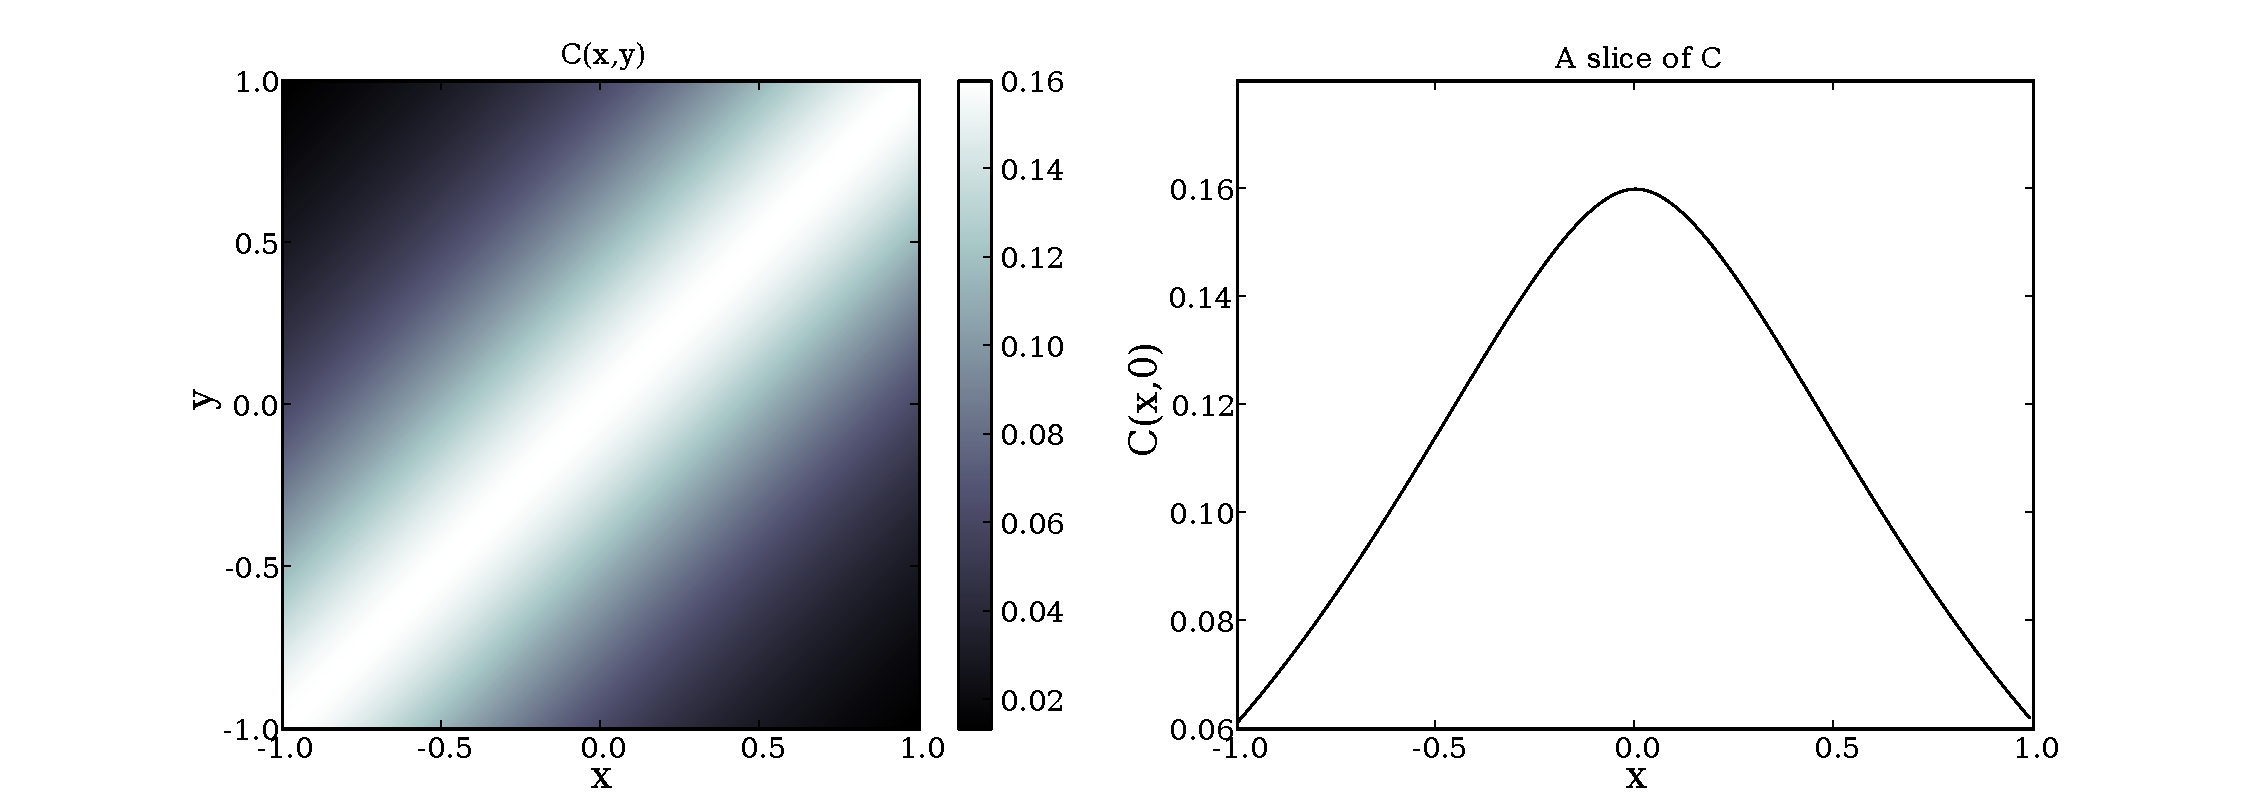
\epsfig{file=figs/cov.pdf,width=15cm}
	\caption{The covariance function generated by {\sffamily `examples/cov.py'}. On the left is the covariance function $C(x,y)$ evaluated over a square: $-1\le x\le 1,\ -1\le y\le 1$. On the right is a slice of the covariance: $C(x,0)$ for $0\le x \le 1$}
	\label{fig:cov}
\end{figure}

GP covariance functions are represented by the class \class{Covariance}, which is essentially a wrapper for ordinary Python functions. In this example we will use the popular Mat\'ern covariance function, which is provided in module \module{cov_funs}. In addition to the two arguments $x$ and $y$, this function takes three tunable parameters: \code{amp} controls the amount by which $f$ may deviate from $M$, \code{diff_degree} controls the smoothness of $f$ (the degree of differentiability), and \code{scale} controls the wiggliness of $f$.

You're free to write your own functions to wrap in \class{Covariance} objects if you want, but not every function of two variables is acceptable as a covariance function. See section \ref{sec:usercov} for more information.

The code shown below will produce an instance of class \class{Covariance} called $C$.
\verbatiminput{../examples/cov.py}

The first argument to \class{Covariance}'s init method, \function{eval_fun}, gives the Python function from which the covariance function will be made. In this case, \function{eval_fun} is \function{Matern}. The extra arguments \code{diff_degree, amp} and \code{scale} will be passed to \function{Matern} every time $C$ is called.

At this stage, the covariance function exposes a very simple user interface. In fact, it behaves a lot like the ordinary Python function it wraps, except that it `memorizes' the extra arguments \code{diff_degree, amp} and \code{scale} so that you don't need to pass them in anymore. Covariance functions' calling conventions are slightly different than ordinary numpy universal functions':
\begin{enumerate}
	\item Broadcasting works differently. If $C$ were a numpy universal function, $C(x,y)$ would return the following array:
	\begin{eqnarray*}
		\begin{array}{ccc}
			C(x_0,y_0)& \ldots& C(x_{N-1},y_{N-1}),
		\end{array}
	\end{eqnarray*}
	but in fact it return a matrix:
	\begin{eqnarray*}
		\begin{array}{ccc}
			C(x_0,y_0)& \ldots& C(x_0,y_{N-1})\\
			\vdots&\ddots&\vdots\\
			C(x_{N-1},y_0)& \ldots& C(x_{N-1},y_{N-1}).
		\end{array}		
	\end{eqnarray*}
	\item You can call it with just one argument; $C(x)$ is interpreted as $C(x,x)$.
\end{enumerate}

Most of the code is devoted to output, which is shown in figure \ref{fig:cov}. It plots the full covariance function over a square, and also the `slice' $C(x,0)$ over an interval. You'll notice that the full covariance function resembles a rounded A-frame tent. The width of this tent controls how tightly nearby evaluations of $f$ are coupled to each other. If the tent is wide, $f(x)$ and $f(y)$ will tend to have similar values when $x$ and $y$ are close-ish to one another. If the tent is narrower, $f(x)$ and $f(y)$ won't be as tightly correlated. The height of the tent controls the overall amplitude of $f$'s deviation from $M$. The sharpness of the tent's peak controls the smoothness of $f$: if the peak is soft, $f$ will be smooth, but if the peak is sharp $f$ will be jagged.

Try playing around with the parameters of \function{Matern} and see how $C$ changes. The only restrictions are that the parameters \code{diff_degree, amp} and \code{scale} have to be positive. If you're brave, try using a covariance function other than \function{Matern}. 

\subsubsection{Instantiating a mean function}\label{subsub:mean}

\begin{figure}
	\centering
		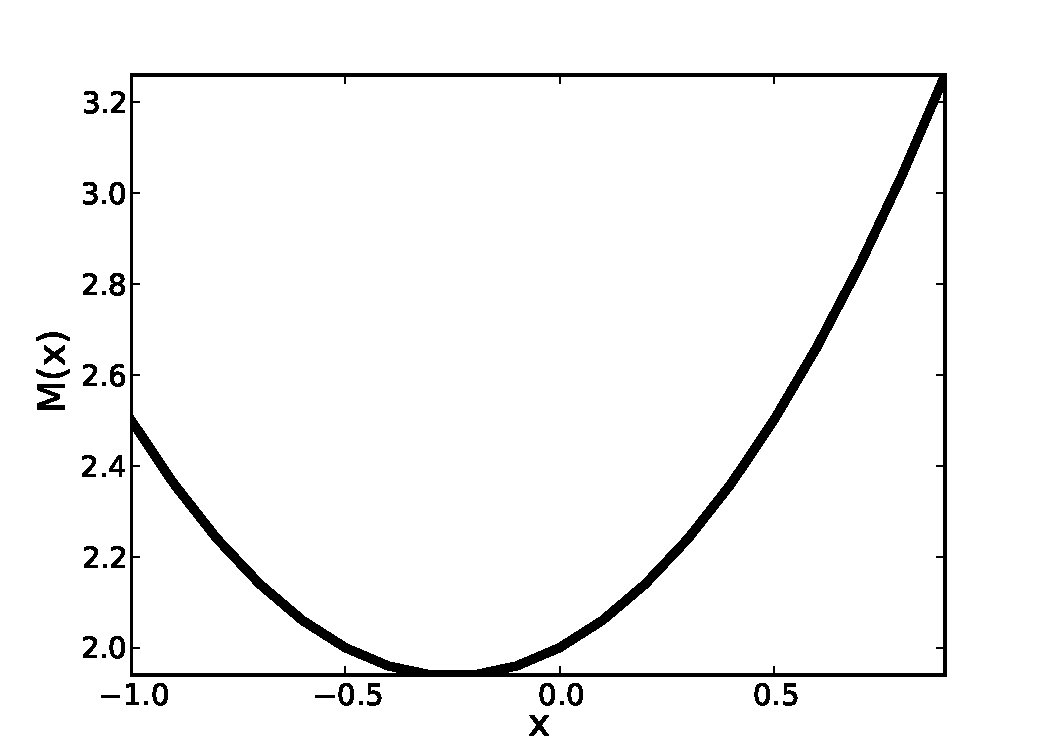
\epsfig{file=figs/mean.pdf,width=10cm}
	\caption{The mean function generated by {\sffamily `examples/meanAndCov.py'}.}
	\label{fig:mean}
\end{figure}

The second component we will generate is the mean function, represented by class \class{Mean}. The mean function of a univariate GP can be interpreted as a prior guess for the GP, so it's a univariate function also. Like \class{Covariance}, \class{Mean} is a wrapper for an ordinary Python function. Unlike the covariance function however, there are no restrictions on the mean function; any function of one variable is fine. We will use the parabola
\begin{equation}
	M(x) = ax^2 + bx + c.
\end{equation}

The following code will produce an instance of class \class{Mean} called $M$:
\verbatiminput{../examples/mean.py}

As with \class{Covariance}, the first argument to \class{Mean}'s init method is the underlying Python function, in this case \function{linfun}. The extra arguments \code{a}, \code{b}  and \code{c} will be memorized and passed to \function{linfun}.
Unlike covariance functions, mean functions broadcast over their arguments in the same way as numpy universal functions, which means that $M(x)$ will return the vector $M(x_0)\ldots M(x_{N-1})$. 

The last part of the code plots $M(x)$ on $-1<x<1$, and its output is shown in figure \ref{fig:mean}. As expected, the plot is a parabola. Mean functions are much less magical than covariance functions, so it won't be as much fun to play with the parameters of \function{linfun}. As stated before, the mean function is just an initial guess for $f$.

\subsubsection{Drawing realizations}\label{subsub:realizations}
\begin{figure}
	\centering
		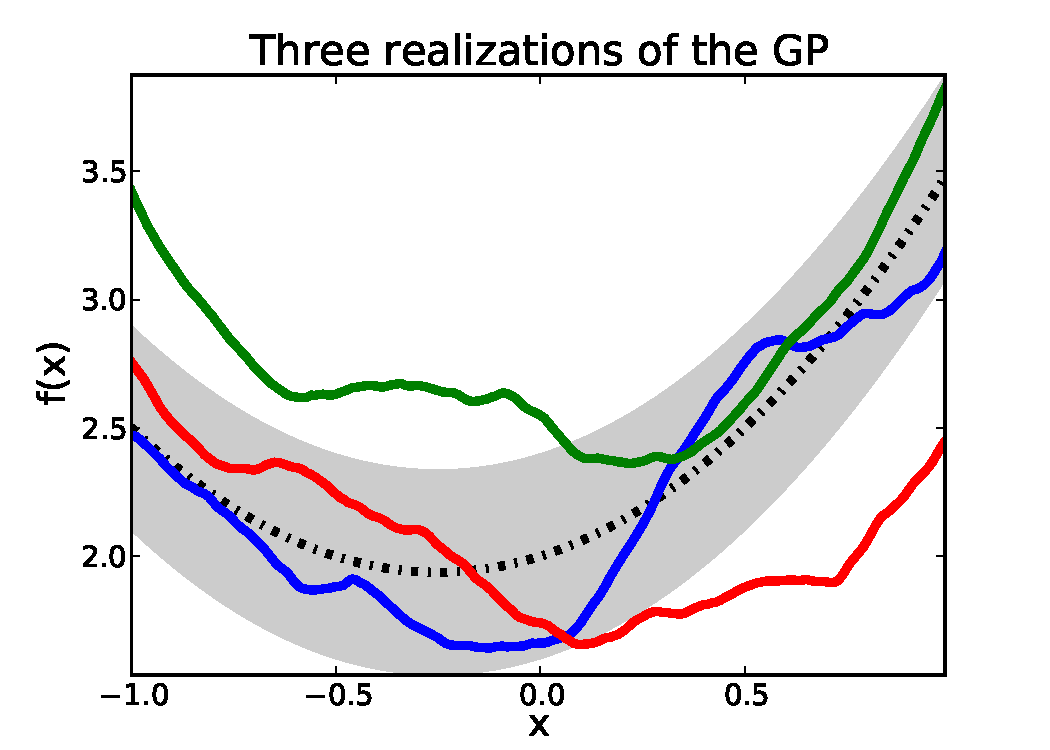
\epsfig{file=figs/realizations.pdf,width=10cm} 
	\caption{Three realizations from a Gaussian process displayed with mean $\pm$ 1 sd envelope. Generated by {\sffamily `examples/realizations.py'}.}
	\label{fig:realizations}
\end{figure}

Finally, let's generate some realizations (draws) from the Gaussian process defined by $M$ and $C$ and take a look at them. The following code will generate a list of instances of class \class{Realization}:
\verbatiminput{../examples/realizations.py}

	The init method of \class{Realization} takes only two required arguments, a \class{Mean} object and a \class{Covariance} object. Each element of \code{f_list} is a Gaussian process realization, which is essentially a randomly-generated Python function. Like \class{Mean} objects, \class{Realization} objects use the same broadcasting rules as numpy universal functions. Typing $f(x)$ will return the vector $f(x_0)\ldots f(x_{N-1})$.

The plotting portion of the code calls the function \function{plot_envelope}, which kind of summarizes the distribution. The dashdot black line in the middle is $M$, and the gray band is the $\pm 1$ standard deviation envelope for $f$, generated by $C$. Each realization is a callable function, and their values over a mesh are plotted superimposed on the envelope. The plot output is shown in figure \ref{fig:realizations}. 

\subsubsection{Experiment!} 

As stated before, the only way you'll be able to use GPs with confidence is by getting some experience with them. Now is a good time experiment with the parameters of the mean and covariance functions. Change parameters of the covariance and mean, see how they look using \file{cov.py} and \file{mean.py} , and try to guess how the realizations will look. See if you're right using \file{realizations.py}.


\section{The role of the covariance function}\label{sec:cov} 

\begin{itemize}
	\item Various visualization methods
	\item Relationship between covariance's shape and properties of $f$
	\item Tour of the library of covariance functions.
\end{itemize}


\section{Nonparametric regression: observing Gaussian processes}\label{sec:observing} 

\begin{figure}
	\centering
		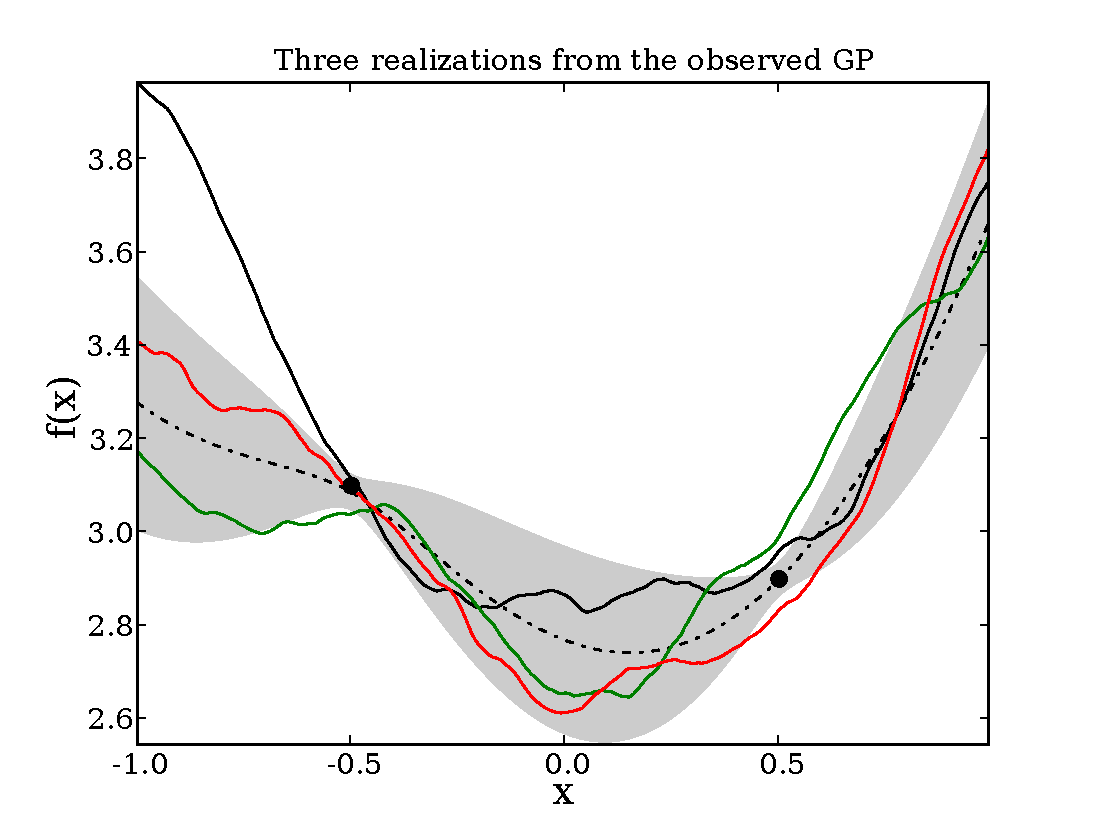
\epsfig{file=figs/obs.pdf,width=8cm}
		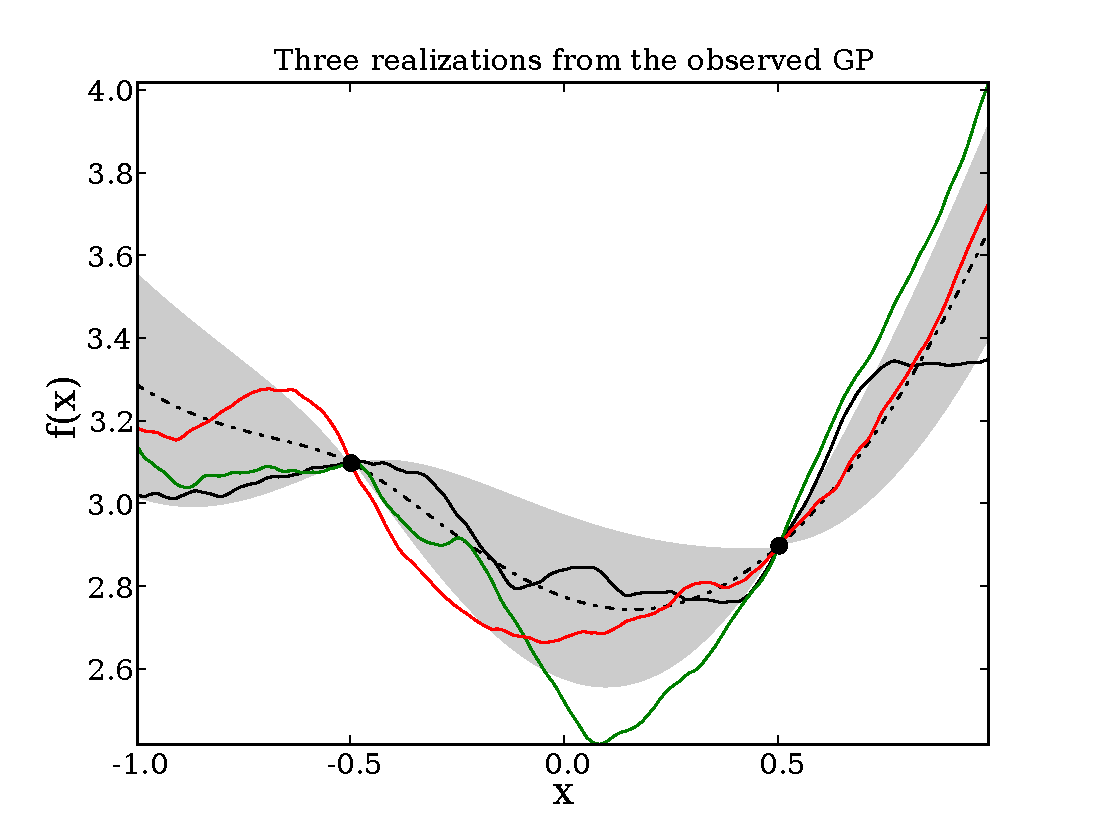
\epsfig{file=figs/cond.pdf,width=8cm}
	\caption{The output of {\sffamily `examples/observations.py'}: the observed (left) and conditioned (right) GP. Note that in the conditioned case, the $\pm$ 1 sd envelope shrinks to zero at the points where the observations were made, and all realizations pass through the observed values.}
	\label{fig:obs}
\end{figure}

Consider the following common statistical situation: You decide on a prior for an unknown function $f$, then you observe the value of $f(x_i)$ at $N$ points, $\{x_i, i=0\ldots N-1\}$, possibly with uncertainty. If the observation error is normally distributed, it turns out that $f$'s posterior distribution given the new information is another Gaussian process, with new mean and covariance functions.

This package provides a function called \function{observe} that allows you to impose normally-distributed observations on your Gaussian process. The following code imposes the observations
\begin{eqnarray}
	f(-.5) = 3.1, & \textup{observation precision}=500\\
	f(.5) = 2.9, & \textup{observation precision}=500
\end{eqnarray}
on the GP defined in \file{mean.py} and \file{cov.py}:
\verbatiminput{../examples/observation.py} 

The function \function{observe} takes a covariance \code{C}  and (optionally) a mean \code{M} as arguments, and essentially tells them that their realizations' values on \code{obs_mesh} have been observed to be \code{obs_vals} with precision \code{obs_taus}. If \code{obs_taus} is \code{None}, \function{observe} assumes that the observation precision was infinite; that is, that the realizations' values on \code{obs_mesh} are known with no uncertainty. Making (or pretending to make) observations with infinite precision is sometimes called \emph{conditioning}, and can be a valuable tool for modifying GP priors; for example, if a rate function is known to be zero when a population's size is zero.

The output of the code is shown in figure \ref{fig:obs}, along with the output with \code{obs_taus=None}, so that the observation precision is infinite. Compare these to the analogous figure for the unobserved GP, figure \ref{fig:realizations}. The covariance after observation is visualized in figure \ref{fig:obscov}. The covariance `tent' has been mashed down at points where $x\approx \pm .5$ and/or $y\approx\pm .5$, which are the values where the observations were made.

\begin{figure}
	\centering
		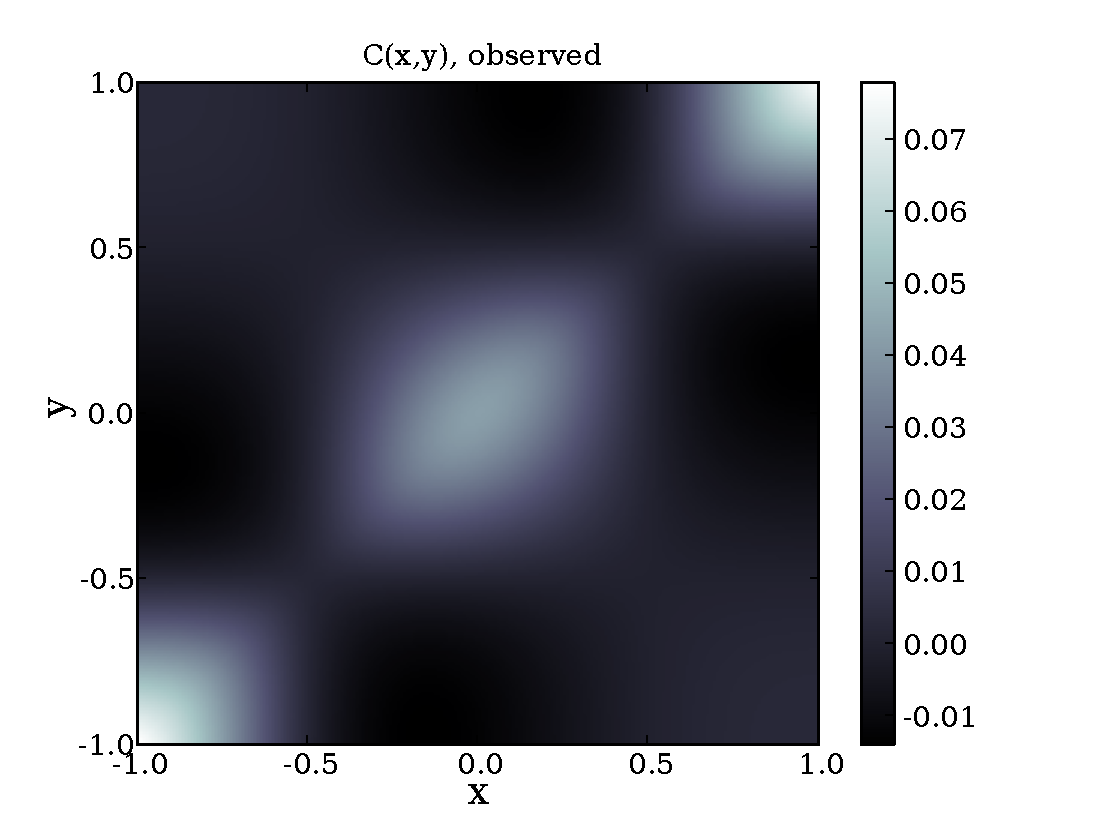
\epsfig{file=figs/obscov.pdf,width=10cm}
	\caption{The covariance function after observation. Compare this with the covariance function before observation, visualized in figure \ref{fig:cov} }
	\label{fig:obscov}
\end{figure}

We finally have the tools to partially reproduce Munch, Mangel and Kottas' results. \textbf{Nonparametric regression with fixed covariance parameters and mean parameters here. Show the stages of the covariance, with realizations: unconditioned, pegged at 0, observed at the datapoints. Note that this is better than MMK's results in some ways and worse in others: We've used Matern and pegged at 0, but haven't allowed covariance parameters to vary. That'll have to wait for section \ref{sec:PyMC}.}



\section{The array aspect and performance}\label{sec:array} 
Conceptually, Gaussian process realizations are random functions, and the parameters of the Gaussian process are functions. To build intuition as quickly as possible, this tutorial has tried to stay faithful to the concepts by focussing on the functional aspects of \class{Covariance}, \class{Mean} and \class{Realization} as long as possible. 

From the programmer's point of view, this was the hard part. Making \class{Realization} act like a function is particularly irritating; its return values have to be evaluated on-demand (lazily) using an algorithm whose expense increases with the number of calls made so far.

You may have noticed by now that \class{Covariance} is a subclass of \class{matrix}, and that \class{Mean} and \class{Realization} are subclasses of \class{ndarray}. That's because these objects are usually represented on a computer as arrays and matrices rather than functions.

Unfortunately, using the array representation of the Gaussian process objects is much faster than using the functional representation we have considered so far. If you need more performance from the Gaussian process than you've been getting, you may need to take a look at this section.

This section will try to introduce you to the array aspect of the GP, while insulating you from as much linear algebra as possible. The first subsection will tell you the bare minimum you need to know to use the array aspect, and the second will give you a hint as to why it works. For the details of the algorithm, see chapter \ref{cha:numerics}.

\subsection{Utilitarian overview: the base mesh}

The init method of \class{Covariance} takes a parameter called \code{base_mesh}, which we haven't talked about yet. The base mesh is where you should put evaluations you know ahead of time you're going to want. The following code recreates the observed GP created in \file{examples/observation.py} and draws a single realization. However, this time a `base mesh' argument is provided.
\verbatiminput{../examples/basemesh.py}

The base mesh will be automatically inherited by the realization $f$. We can do a few things now that we couldn't do before.

\subsubsection{Indexing and slicing}\label{subsub:indexslice}
First, try typing the following command into the Python prompt, and you'll get the output below:
\begin{verbatim}
In [3]: print C
Gaussian process covariance
functional aspect: <function Matern at 0x496f4b0>
matrix aspect: ([[  7.78885868e-02,   6.60273508e-02,   4.99286671e-02,
                    3.22586177e-02,   1.53194936e-02,   1.48744121e-03,
                   -7.22296442e-03,  -1.18739011e-02,  -1.37398672e-02,
                   -1.36941495e-02,  -1.23668617e-02,  -1.02279152e-02,
                   ...
\end{verbatim}
$C$'s new `matrix aspect' is just $C$ evaluated on its base mesh. Try typing \code{print M} and \code{print f} into the prompt also. 

$C$ can still be called like a function, but now it can be indexed and sliced like a matrix too:
\begin{verbatim}
In [11]: C(2.,3.)
Out[11]: matrix([[ 0.06014876]])

In [12]: C[3,:5]
Out[12]: matrix([[ 0.03225862,  0.03155917,  0.02869263,  0.02249194,  0.01228326]])

In [13]: isinstance(C,matrix)
Out[13]: True
\end{verbatim}
Similarly, $f$ and $M$ can still be called like functions, but now they can be indexed and sliced like arrays:
\begin{verbatim}
In [14]: M(3)
Out[14]: array(12.506241348839085)

In [15]: f(3)
Out[15]: array(12.492415530964509)

In [16]: M[:5]
Out[16]: array([ 3.27805131,  3.22089361,  3.18082649,  3.1518305 ,  3.12490149])

In [17]: f[:5]
Out[17]: array([ 3.5334958 ,  3.46852459,  3.47008632,  3.3340304 ,  3.14679477])

In [18]: isinstance(M,ndarray)
Out[18]: True

In [19]: isinstance(f,ndarray)
Out[19]: True
\end{verbatim}

As you may have noticed, slicing (getting values from the array aspect) is much, much faster than calling (getting values from the functional aspect). \textbf{This part may not be true if you use Bach and Jordan's algorithm for the Cholesky decompositions of observation covariances, but a lesser method to handle the base mesh. The only reason for the base mesh may now be Metropolis algorithms and measure continuity in MCMC. Try to sort this out.} If performance is a concern, you should make your base mesh include every value you're ever going to want, so that you don't have to make many calls at all. If that's not possible, you should keep the number of calls you make to a minimum. If you absolutely have to make a lot of calls but you still need high performance, consider a Fourier representation.
 
\subsubsection{Computing log-probabilities of realizations}\label{subsub:logp}
This module provides a function called \function{GP_logp} for computing the log probability density of the evaluation of a realization $f$ on a base mesh, with respect to a mean function $M$ and a covariance function $C$. Try it out:
\begin{verbatim}
In [20]: GP_logp(f,M,C)
Out[20]: 39.2993852418

In [21]: GP_logp(2.*f,M,C)
Out[21]: -4667.56968213
\end{verbatim}
It looks plausible that $f$ is a realization from the GP defined by $M$ and $C$, but much less plausible that $2f$ is such a realization. This makes sense; $f$ really is a realization from that GP, but $2f$ would be way too far away from $M$ (see the $\pm$ 1 sd bands in figure \ref{fig:obs}, and imagine how ridiculous the realizations would look if they were doubled in amplitude).

If \function{GP_logp} is called with a realization $f$ that is way too ridiculous to ever have arisen from the GP, it returns \code{-Inf}.

It's important to note that the log-probabilities of two realizations should only be compared to one another if the realizations have the same base mesh. Doing otherwise is like comparing area to volume.

\subsubsection{Specifying realizations' values on the base mesh}\label{subsub:force}

The init method of \class{Realization} takes an argument we haven't used yet, called \code{init_base_array}. It allows us to force the realization to take particular values on the base mesh; that is, it allows us to force an array aspect on the realization. This is useful for proposing values in MCMC. We will defer further discussion of this feature until we need it in section \ref{sec:PyMC}. 

\subsection{The theory behind the array aspect} 
The Gaussian process generalizes the multivariate normal distribution from vectors to functions, just like the multivariate normal distribution generalizes the univariate normal distribution from scalars to vectors. The progression is as follows:
\begin{equation}
    \begin{array}{ll}
        y\sim\textup N(\mu,V): & \textup{$y$, $\mu$, $V$ are scalars}\\\\
        \vec y\sim\textup N(\vec \mu,C): & \textup{$\vec y$ and $\vec \mu$ are vectors, $C$ is a matrix}\\\\
        f\sim\textup{GP}(M, C): & \textup{$f$ and $M$ are functions of one variable, $C$ is a function of two variables}
    \end{array}
\end{equation}

One of the really nice things about this extended family of distributions is that it's easy to marginalize. For example, each element of a vector with a multivariate normal distribution has a univariate normal distribution:
\begin{eqnarray*}
    \vec y\sim\textup N(\vec \mu,C)\\
	\Rightarrow \vec y_i\sim\textup N(\vec \mu_i,C_{i,i}),
\end{eqnarray*}
and any subvector of a vector with a multivariate normal distribution has a multivariate normal distribution:
\begin{eqnarray*}
    \vec y\sim\textup N(\vec \mu,C)\\
	\Rightarrow \vec y_{i_1\ldots i_2}\sim\textup N(\vec \mu_{i_1\ldots i_2},C_{i_1\ldots i_2,i_1\ldots i_2}),
\end{eqnarray*}

This marginalizability applies to GP's as well. If $\vec x$ is a vector of values (a base mesh),
\begin{equation}
	\begin{array}{l}
		f\sim\textup{GP}(M, C)\\\\
		\Rightarrow f(\vec x) \sim\textup N(M(\vec x), C(\vec x,\vec x)).
	\end{array}
\end{equation}
In other words, the array aspect of a Gaussian process \class{Realization} has a multivariate normal distribution. Its mean is the array aspect of $f$'s associated \class{Mean} function, and its covariance is the matrix aspect of $f$'s associated \class{Covariance} function. You can probably start to see why this fact is important for working with GPs on a computer. For the details, see chapter \ref{cha:numerics}. 

\section{Higher-dimensional GPs}\label{sec:highdim} 
\textbf{Under construction}
Any time you pass an array into an init method or evaluate a GP object on an array, the convention is that the array's last index iterates over spatial dimension. So if you wanted to evaluate a covariance function $C$ on the ordered pairs $(0,0)$, $(0,1)$, $(1,0)$ and $(1,1)$, you could pass in the following two-dimensional array:
\begin{verbatim}
[[0,0]
 [0,1]
 [1,0]
 [1,1]]
\end{verbatim}
or the following three-dimensional array:
\begin{verbatim}
[[[0,0]
  [0,1]],

  [1,0]
  [1,1]]]
\end{verbatim}
Either is fine, since in both the last index tells you which element of the ordered pair to use.

\textbf{A spatial example in 2d}

% chapter basics (end)


\chapter{Tutorial II: More advanced topics}\label{cha:adv} % (fold)

\section{Incorporating Gaussian processes in larger probability models with PyMC}\label{sec:PyMC} 
\textbf{This section will use Munch, Mangel and Kottas' model and data soon.}

This section will show you how to build statistical models that go beyond simple nonparametric regression. You'll want to do this eventually, as there are many inferential problems in ecology and other fields where a Gaussian process makes sense that can't be cast as simple nonparametric regressions. 

We'll present a modest extension of the nonparametric regression here: we'll follow Munch, Mangel and Kottas by putting `hyperpriors' on the parameters of the mean and covariance functions, as well as the observation precision, and infer them along with $f$. We'll use a modest extension rather than a flamboyant one so as not to obscure ideas, but I hope it whets your appetite.

We will implement the extension using PyMC 2.0, which provides very general support for specification and manipulation of Bayesian statistical models, with emphasis on Markov Chain Monte Carlo methods. PyMC is intended to provide at least basic support for any statistical model, and clear avenues for users and contributors to improve that support for specialized submodels. Before proceeding, you should familiarize yourself with the PyMC 2.0 documentation, available from the project homepage at \citetitle[trichech.us/?page_id=4]{www.trichech.us}.

\begin{figure}
	\centering
		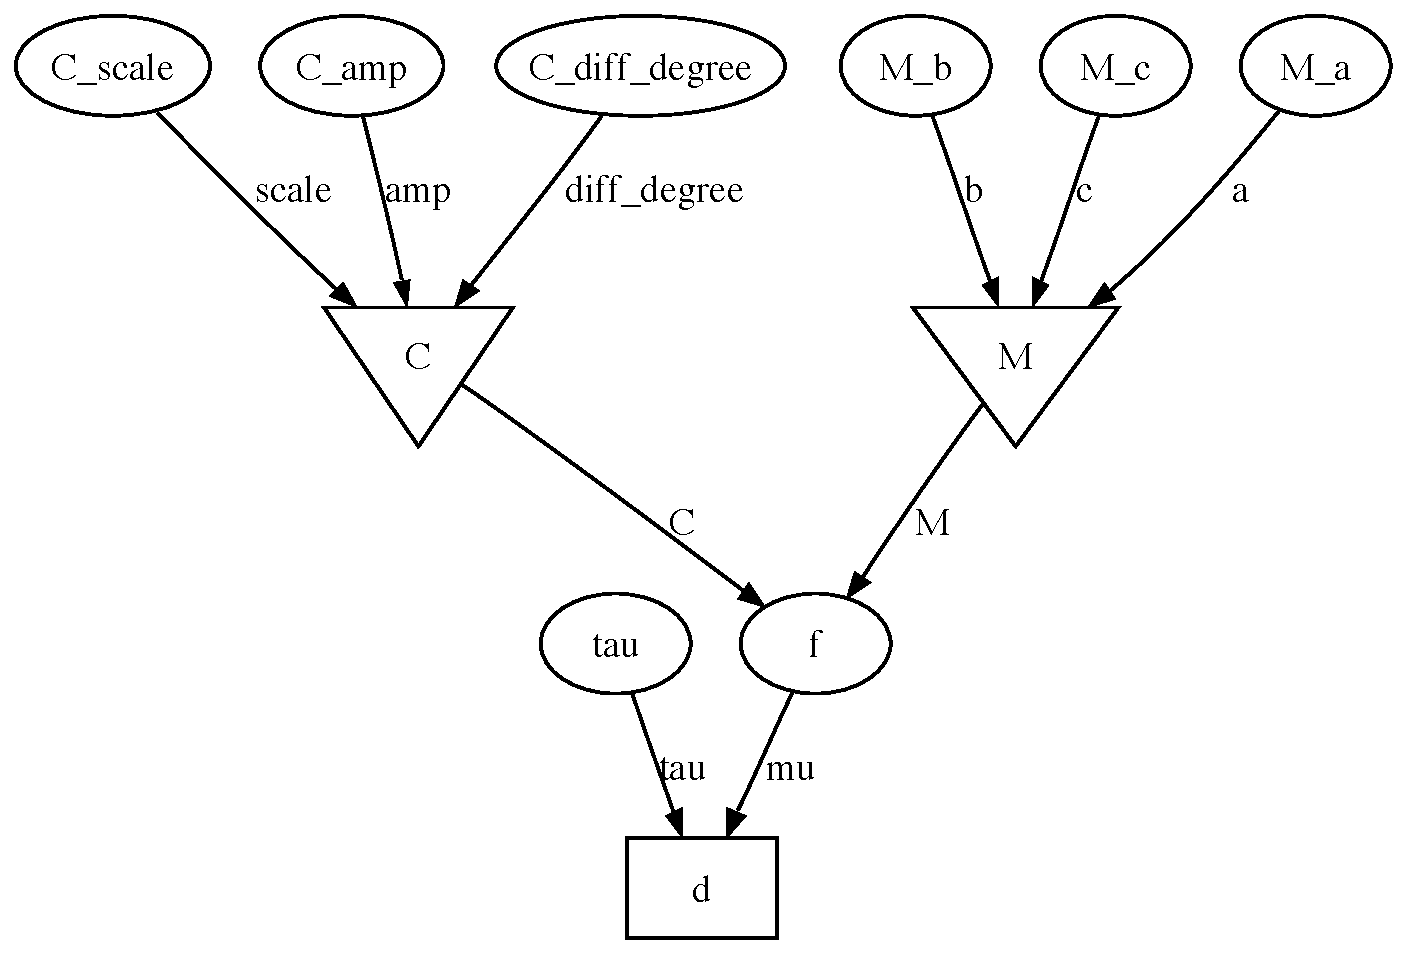
\epsfig{file=figs/unobservedModel.pdf, width=10cm}
	\caption{The PyMC-generated directed acyclic graph representation of the extended nonparametric regression model, given in section \ref{sec:PyMC}. Ellipses represent \class{Parameter} objects (variables whose values are unknown even if their parents' values are known), triangles represent \class{Node} objects (variables whose values can be determined if their parents' values are known), and rectangles represent \class{Parameter} objects with the \member{isdata} flag set to \member{True} (\class{Parameter} objects whose values happen to be known). Arrows point from parent to child, and arrow labels show the name assigned to the parent by the child. For instance, \class{C} considers \class{C_amp} to be its `\class{amp}' parameter.}
	\label{fig:unobservedModel}
\end{figure}

The probability model we'll use, which is like Munch, Mangel and Kottas' nonparametric regression model, is as follows:
\begin{equation}
	\label{eqn:npregression}
	\begin{array}{ll}
		d_i|f,\tau\stackrel{{\tiny ind}}{\sim} \textup N(f(x_i), \tau),&i=1\ldots N\\\\
		f|a,b,c,\nu,\phi,\alpha\sim\textup{GP}(M(a,b,c),C(\textup{amp} ,\textup{diff\_degree} ,\textup{scale}))&\\\\
		\{a,b,c,\textup{amp} ,\textup{diff\_degree} ,\textup{scale},\tau\} \sim \textup{priors}.
	\end{array}
\end{equation}
Our version of the model is slightly different from Munch, Mangel and Kottas' in that we use the Mat\'ern covariance function, conditioned using the \function{observe} function so that $f(0)$ is guaranteed to be equal to zero.

The statistical model is visualized as a directed acyclic graph in figure \ref{fig:unobservedModel}. Its translation to a PyMC probability model is given in \file{examples/PyMC_model.py}. The code is a bit long to quote here, but I will discuss the sections involving Gaussian process objects. 

First, take a look at the following portions:
\begin{verbatim}
@node
def C(eval_fun = Matern, base_mesh = x, diff_degree=C_diff_degree, amp=C_amp, scale=C_scale):
    return Covariance(eval_fun, base_mesh, diff_degree=diff_degree, amp=amp, scale=scale)

...

@node
def M(eval_fun = linfun, base_mesh = x, a=M_a, b=M_b, c=M_c):
    return Mean(eval_fun, base_mesh, a=a, b=b, c=c)

\end{verbatim}
This code declares two nodes, \var{M} and \var{C}, whose \member{value} attributes are actually a \class{Mean} instance and a \class{Covariance} instance, respectively. PyMC nodes are variables whose values are known if their parents' values are known.
\textbf{You may want to eliminate the base mesh, and tack an evaluation node onto f that will only get queried during tallies. That will save a lot of Matern evaluations.}

Now, look at this line:
\begin{verbatim}
f = GaussianProcess(M=M, C=C, name='f')
\end{verbatim}
As explained in the code, this is shorthand for the more standard PyMC notation
\begin{verbatim}
@parameter(__class__ = GaussianProcess)
def f(value=Realization(M,C), M=M, C=C):

    def logp(value, M, C):
        return GP_logp(value,M,C)

    def random(M, C):
        return Realization(M,C)
\end{verbatim}
PyMC parameters are random variables, which are variables whose values are unknown even if their parents' values are known. The value of \var{f} is an actual \class{Realization} object whose log-probability is computed using the \function{GP_logp} function from this package. Its \method{random} method returns a new \class{Realization} object, since \class{Realization}s are really just draws from Gaussian process distributions.

The parameter \var{f} will be an instance of a special \class{Parameter} subclass called \class{GaussianProcess}. This subclassing is done to help \class{Sampler} figure out which sampling method can best handle it. 

The following standard PyMC code declares the observation precision (which is unknown) and the data, which depends directly on the observation precision and $f$:
\begin{verbatim}
@parameter
def tau(value=500., alpha = 1., beta = 500.):
    """tau ~ gamma(alpha, beta)"""
    if value<=0.:
        raise LikelihoodError
    return flib.gamma(value, alpha, beta)

@data
def d(value=array([3.1, 2.9]), x=obs_x, mu=f, tau=tau):
    """
    d ~ N(f(obs_x), tau)

    Note that because of f's base mesh:
        f[5] = f(-.5)
        f[-5] = f(.5),
    so
        [f[5], f[-5]] = f(obs_x).
        
    The array aspect is therefore used for value access,
    because it's much faster.
    """
    mu_array = array([mu[5],mu[-5]])
    return flib.normal(value, mu_array, tau)
\end{verbatim}

Finally, the following line declares a special Gibbs sampling method to handle \var{f}:
\begin{verbatim}
S = ObservedGPGibbs(f=f, M=M, C=C, obs_mesh=obs_x, obs_taus=tau, obs_vals=d)
\end{verbatim}
If you comment this line out, \class{Sampler} will assign the default \class{GPMetropolis} sampling method to \var{f} instead of \class{ObservedGPGibbs}. Running \file{examples/MCMC.py} will run the MCMC loop and plot output; some of its output using \class{GPMetropolis} and \class{ObservedGPGibbs}. is shown in \ref{fig:MCMCOutput}. 

\begin{figure}
	\centering
		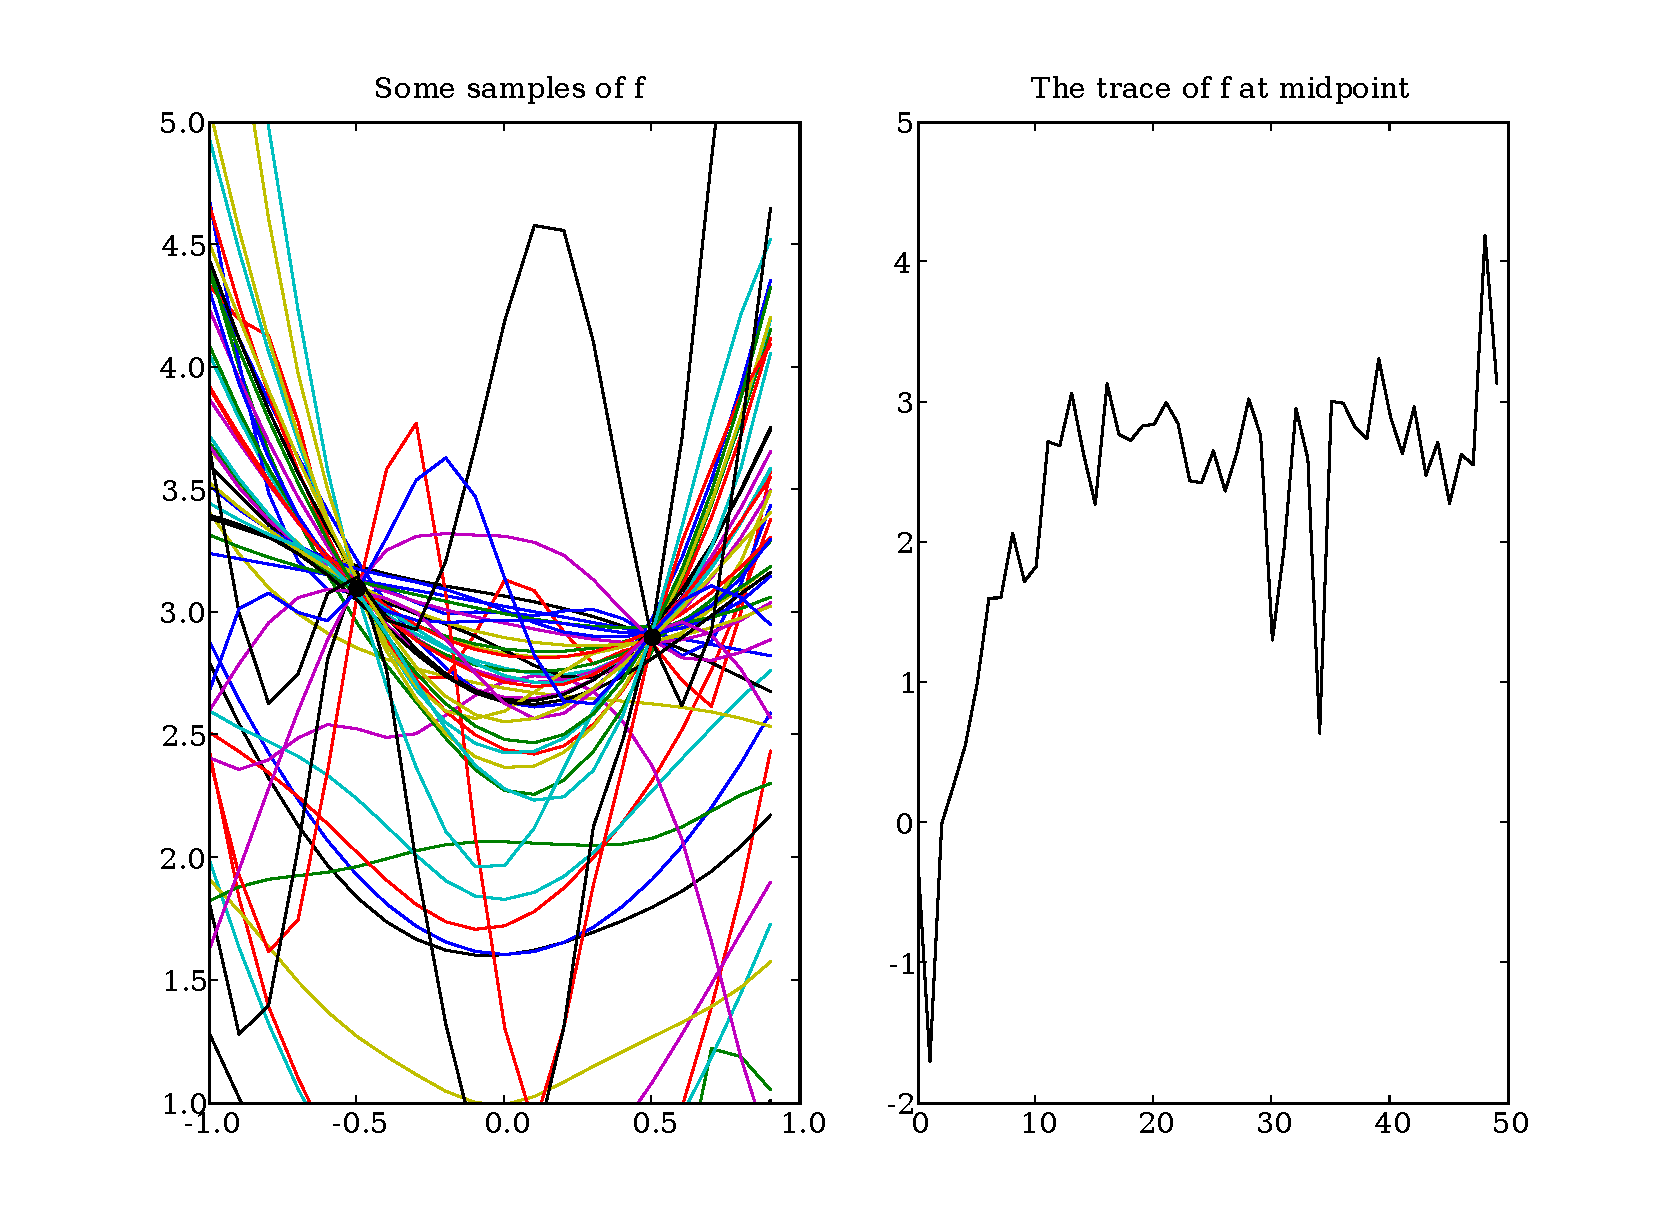
\epsfig{file=figs/metroSamples.pdf,width=10cm}
		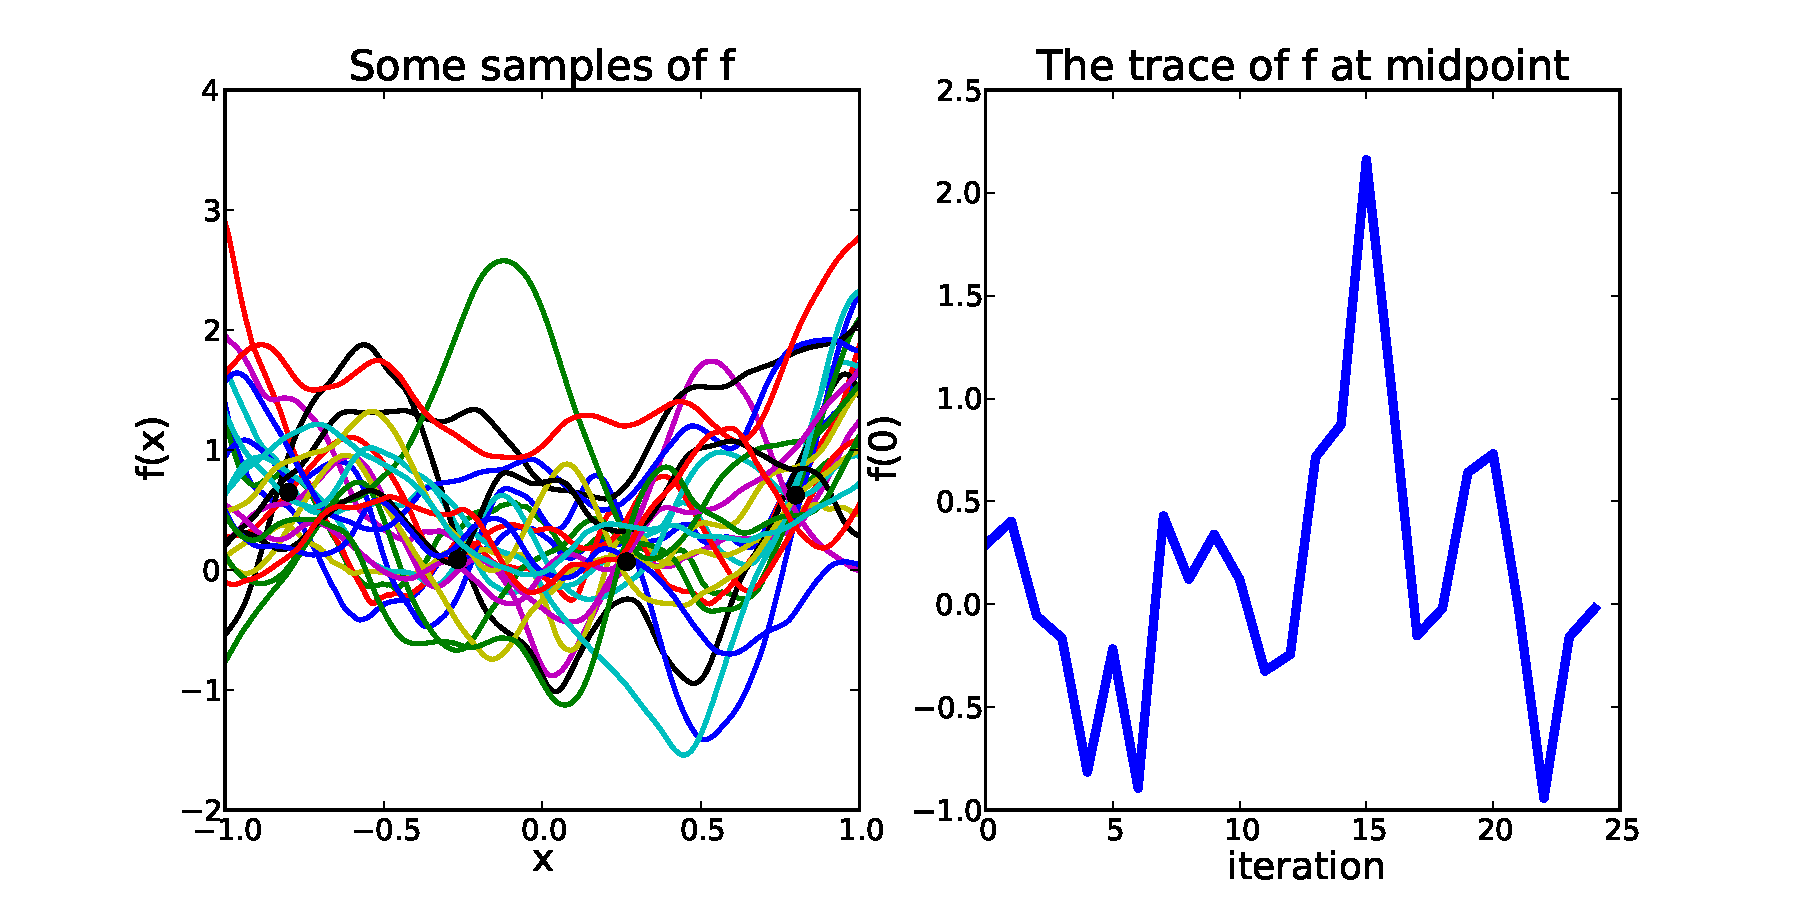
\epsfig{file=figs/gibbsSamples.pdf,width=10cm}		
	\caption{The output of {\sffamily `examples/MCMC.py'} using the default \class{GPMetropolis} sampling method (above) and a user-declared \class{GPGibbs} sampling method (below). You can see that the Metropolis samples take a while to `burn in' and find the dense part of the posterior distribution, but the Gibbs samples jump right to their dense support and explore it more quickly. However, the Metropolis sampler is cheaper and has `gentler' numerical properties, and you don't have to declare anything to use it. \textbf{Think about whether this is true with Bach and Jordan's method.} In applications, you'll usually want to try both.}
	\label{fig:MCMCOutput}
\end{figure} 

\section{Integrals, derivatives and transforms: linear operations and constraints}\label{sec:linop} 

\textbf{Not implemented yet. Maybe try to make a LinearOperator class. Define linear operations, talk about derivatives, integrals and Fourier transforms, how you can easily find their distribution. You can constrain the value of any linear operation, or softly constrain it. This is handy for building covariance functions. Introduce the \var{lintrans} argument. Maybe this shouldn't go in the tutorial.}



\section{Fourier representations, splines and convolutions}\label{sec:approx} 
Good if you need to make lots of calls, it's hard to establish a base mesh. Need to see how much can be implemented in time.

\subsection{Fourier representations}\label{sub:fourier}
\begin{itemize}
	\item Pros:
	\begin{itemize}
		\item Easy to go back and forth between Fourier and standard GP.
		\item Very solid and well-established theory.
		\item Straightforward to manipulate smoothness and wiggliness properties.
		\item Can often diagonalize covariance.
	\end{itemize}
	\item Cons:
	\begin{itemize}
		\item Harder for some people to visualize.
		\item Less standard in the field.
	\end{itemize}
\end{itemize}

\subsection{Splines}\label{sub:splines}
\begin{itemize}
	\item Pros \& cons: Need to ask Angela
\end{itemize}

\subsection{Convolutions}\label{sub:convolutions}
Need to look at Paciorek's thesis, see how much could be implemented in time.



\section{Writing your own covariance functions}\label{sec:usercov} 
If you want to write your own covariance function at some point, this module provides a function called \function{isPosDef} that can help you determine if your function is acceptable. It tests if a function is positive definite using Bochner's theorem. Also, \class{Covariance} will raise an error if it's able to determine that its underlying function is unacceptable, but it won't catch every unacceptable function. 

Three simple rules always apply to covariance functions, and keeping them in mind will reduce the amount of trial and error you have to go through:
\begin{itemize}
	\item $C(x,y)=C(y,x)$ for any $x$ and $y$.
	\item $C(x,x) \ge 0$ for any $x$.
	\item $C(x,x)\ge C(x,y)$ for any $x$ and $y$.
\end{itemize}

The theoretical condition is that the covariance has to be a symmetric nonnegative-definite function: its evaluation on any finite mesh has to be a symmetric nonnegative-definite matrix, which is a symmetric matrix whose eigenvalues are all nonnegative.



% chapter adv (end)


\chapter{Numerics: the nitty gritty details}\label{cha:numerics} % (fold)
For the time being, this section is just my game plan. I'd like the numerics to be really fast and robust, so that this becomes something people can really feel comfortable using. 

Terminology:
\begin{itemize}
	\item $b$: The base mesh. Note that no matter how efficient the calling algorithm gets, the base mesh will still be essential for comparing the log-probability of two realizations. You can't get rid of the base mesh altogether, though it'll hopefully not be a performance issue eventually.
	\item $o$: The observation mesh.
	\item $l$: The linear transformation relating the observation to the evaluation of $f$.
	\item $d$: The observation values.
	\item $\tau$: The observation precisions.
	\item $x$ and $y$: Some random set of points on which the user calls an object.
	\item $M$: A mean function.
	\item $C$: A covariance function.
	\item $f$: A realization.
	\item $b_f$: The internal mesh of realization $f$ (the distinction between base and observation is irrelevant).
	\item $M_f$: The internal mean function of $f$
	\item $C_f$: The internal covariance function of $f$
\end{itemize}

\section{Shopping list}\label{sec:shoppingList} 
\begin{itemize}
	\item Algorithm 1: A fast Cholesky decomposition which is OK with putting zeros on the diagonal. Prime candidate is Bach and Jordan's method, which could just be wrapped using f2py and called from Python. It outputs a smart low-rank Cholesky decomposition using $o$ and $d$.
	
	The primary drawback (which is also a feature) is that it only does the Cholesky decomposition with a data vector input. That means the base covariance can't be Choleskified except in the presence of a data vector. That'll require a rethinking of the algorithms... in particular, the need for algorithm 2 will go away because there'll be no point downdating the Cholesky factorization of the base mesh, because it can't be taken until it's needed. Also, algorithm 4 will probably be out of the question.
	
	It may be best to use a hybrid approach: Compute the terms involving the inverses when observations are made using Bach and Jordan's method, but store the base mesh as a standard Cholesky decomposition, possibly using LU or LDU for extra robustness against zero diagonals.
	
	The alternative is to keep the base mesh unfactored, and only factor it when log-probability densities are computed. The disadvantages to this would be: A standard Cholesky would be needed for drawing random values (because no data would be available), and it would be hard to guarantee that the log-probabilities of different realizations was being assessed with respect to the same measure.
	
	\item Algorithm 2: An efficient (linear-order) Cholesky downdating algorithm that doesn't require multiplying out the outer product.
	\item Algorithm 3: Takes a triangular matrix $L$ and computes $L^{-1}B$ for some $B$. If $L$ has zeros on the diagonal, it should still try its best, and only raise an error if $B$ has a nontrivial component in a forbidden eigendirection.
	\item Algorithm 4: The things described in section \ref{sec:succObs}. This shouldn't be a big deal, it only requires keeping track of blocks.

\section{Instantiation of the covariance function}\label{sec:covInstant} 
When the covariance function is instantiated, the following matrices will be stored:
\begin{itemize}
	\item The evaluation $C(b,b)$
	\item $L$, the Cholesky factorization of $C(b,b)$.
\end{itemize}
$L$ needs to be computed using an algorithm that is tolerant the fact that $C$ may have some eigenvalues that are very close to zero, or even identically zero (ie, covariances constructed from finite Fourier series). Call this algorithm 1.

\section{Observation of the mean and covariance functions}\label{sec:obsNumerics} 
The matrix aspect of the covariance and the array aspect of the mean need to be updated as follows:
\begin{eqnarray*}
	C(b,b) -= C(b,o) l^T (l(C(o,o) + \tau^{-1})l^T)^{-1} l C(o,b)\\
	M(b) -= C(b,o) l^T (l(C(o,o) + \tau^{-1})l^T)^{-1} (d-M(o)).
\end{eqnarray*}

Instead of inverting the kernel, its Cholesky factorization should be computed and stored using algorithm 1. 

The terms of the form $B K_o^{-1} A$ should be computed using algorithm 2, which leverages the Cholesky factorization and is aware that $K_o$ may not be invertible. In particular, it should invert one Cholesky factor onto $l$ and invert the other onto $A$. If it finds that a Cholesky matrix is singular, it should ensure that the matrix onto which it is being inverted has no component along the degenerate eigendirections.

The covariance should be updated using algorithm 3, which is a downdating algorithm that is sensitive to the fact that $C$ needs to remain positive definite. This will require a generalization of the algorithms that are currently available.

$C$ should store a copy of $K_o=(l(C(o,o) + \tau^{-1})l^T)$ and its quasi-Cholesky factorization $L_o$. M should store a copy of $L_o^{-1}(d-M(o))$, which may contain some kind of infinity, somehow.

\section{Successive observations}\label{sec:succObs}
Successive observations need to be allowed. Say $M$ and $C$ have been observed on $o_1$, and now they're going to be observed on $o_2$. They could just make an internal copy of themselves, and consider that their new unobserved evaluation function. Then it would just be business as usual to update the array aspect. Unfortunately, I think that's highly suboptimal. 

Here's the goal of algorithm 4: You know $C(b,b)$, $C(b,o_1)$, $C(o_1,o_1)$, $L(o_1,o_1)^{-1}C(o_1,b)$, $M(b)$, $M(o_1)$ and $L(o_1,o_1)^{-1}(d_{o_1} - M(o_1))$. You need to compute $C(b,o_2)$, $C_{o_1,o_2}$ and $C_{o_2,o_2}$ the old-fashioned way. From those, you want to compute the following efficiently:
\begin{itemize}
	\item $L([o_1,o_2]^T,[o_1,o_2])$, then
	\item $L([o_1,o_2]^T,[o_1,o_2])^{-1} C([o_1,o_2]^T,b)$ and
	\item $L([o_1,o_2]^T,[o_1,o_2])^{-1} ([d_{o_2}, d_{o_1}]^T - [M(o_1), M(o_2)]^T)$.
\end{itemize}
Parts of these products can be skipped, since the upper part of the inverse of $L$ is the inverse of the upper part. That means the problem really comes down to: recomputing the Cholesky factorization efficiently, and solving the system efficiently when you already know some components of the solution.

\section{Calls to observed means}\label{sec:obsMeanCalls} 
If the user requests $M(x)$, the following should happen:
\begin{itemize}
	\item $M(x)$ is computed directly from the mean function (without regard for the observations).
	\item $M(x) - C(x,o) l^T K_o^{-1} (d-M(o))$ should be computed and returned. If the term $L_o^{-1}(d-M(o))$ has been stored, this requires algorithm 3.
\end{itemize}
$M(x)$ should not learn anything from this experience.

\section{Calls to observed covariance functions}\label{sec:obsCovCalls} 
If the user requests $C(x,y)$, the following should happen:
\begin{itemize}
	\item $C(x,y)$ is computed directly from the mean function (without regard for the observations).
	\item $C(c(x,y),c(x,y)) - C(c(x,y),o) l^T K_o^{-1} l C(c(x,y),o)$ should be computed, sliced and returned. The sqrt of the right-hand term can be computed by algorithm 2, and the downdating done by algorithm 3. If $x$ and $y$ share elements, redundant computation should be avoided.
\end{itemize}
$C$ should also not learn anything from this experience.

\section{Calls to realizations}\label{sec:callsToRealizations}
A realization starts with an internal mesh $b_f$, which combines its base mesh and all the points on which its value has been observed to date. It also has internal mean and covariance objects called $M_f$ and $C_f$, which have been observed on $b_f$.

Now the user queries $f(x)$ for a new vector $x$. The following should happen:
\begin{itemize}
	\item Any elements of $x$ that have already been computed are set aside.
	\item $M_f(x)$ and $C_f(x)$ are computed, and from those a value for $f(x)$ is drawn. $C_f$ should be decomposed using algorithm 1.
	\item $M_f$ and $C_f$ are observed on $x$ using the new values $f(x)$, with infinite precision. $x$ is appended to $b_f$.
	\item The new $f(x)$ is returned to the user.
\end{itemize}
Using an internal mean and covariance object saves code duplication, which is good for everyone.
	
\end{itemize}

% chapter numerics (end)

\chapter{API reference}\label{cha:reference} 

Doxygen-style class reference here.


\end{document}
